% ============================================================
% CHAPTER 4: BEST INPUT REPRESENTATION
% Draft status: full skeleton with real numbers where available.
% Prose is intentionally skeletal — expand per section notes.
% Figures marked [HAVE] exist; [NEED] require new inference/plots.
% ============================================================

\chapter{Best Input Representation}
\label{ch:input-repr}

% --- SECTION INTRO NOTE ---
% 1 paragraph: frame the question as "before the transformer sees anything,
%   choices have already been made." Name the six axes: T1, T1-a, T1-b, D01,
%   D02, D03. State the two lenses: (1) performance (what helps?) and (2)
%   interpretability (what does the gap reveal about the physics?).
% Mention that the chapter baseline (Table~\ref{tab:ch4-baseline}) flows
%   forward into every subsequent chapter.

Before the transformer processes a single attention operation,
several choices have already shaped the information available to it:
whether each particle token carries an additional explicit identity label or only
its four-vector with $p_t$ and $E$, $\eta$ and $\phi$ (T1), and if it does carry the Particle ID
how that label is encoded (T1-a, T1-b),
which kinematic components are included (D01),
whether missing transverse energy is present as an additional token (D02),
and in what order the tokens arrive (D03).
This chapter asks which of these choices matter, and why.
The experimental programme consists of two sweeps:
Experiment~4A varies the tokenizer family and PID encoding,
and Experiment~4B varies the feature set, MET inclusion, and token ordering.
All other axes are held at the canonical defaults defined in
Chapter~\ref{ch:workbench}.

% ============================================================
\section{Tokenizer family and PID encoding (Exp.\ 4A)}
\label{sec:exp4a}
% ============================================================

% --- SECTION INTRO NOTE ---
% 1 short paragraph: the core question is whether particle identity is
%   recoverable from kinematics alone. State that we test three families
%   (raw, identity, binned) and, within identity, sweep T1-a (pid_mode)
%   and T1-b (id_embed_dim). Refer to Table~\ref{tab:exp4a}.

\begin{table}[h]
\centering
\small
\begin{tabular}{lllr}
\toprule
Factor & Values & Applies to & $n_\text{configs}$ \\
\midrule
T1 — Tokenizer family & \texttt{raw} & all & 1 \\
                       & \texttt{binned} & all & 1 \\
                       & \texttt{identity} & — & — \\
\quad T1-a — PID mode & \texttt{one\_hot}, \texttt{fixed\_random}, \texttt{learned} & identity & 3 \\
\quad T1-b — PID dim  & 8, 16, 32 & identity & 3 \\
\midrule
\multicolumn{3}{l}{Unique configurations} & 11 \\
\multicolumn{3}{l}{Seeds per configuration} & 3 \\
\multicolumn{3}{l}{\textbf{Total runs}} & \textbf{33} \\
\bottomrule
\end{tabular}
\caption{Experiment 4A sweep design.
All axes not listed are held at the canonical defaults (Chapter~\ref{ch:workbench}).
D01\,=\,\texttt{[0,1,2,3]}, D02\,=\,\texttt{false}, D03\,=\,\texttt{input\_order}.}
\label{tab:exp4a}
\end{table}

% -------------------------------------------------------
\subsection{Tokenizer family comparison}
\label{sec:exp4a-family}
% -------------------------------------------------------

% --- NOTE ---
% Core argument (2–3 sentences): identity outperforms raw by +0.031 AUROC
%   and binned by +0.040. The ROC curves confirm this is a uniform lift,
%   not threshold-specific. The training dynamics (Fig~\ref{fig:val-auroc-tokenizer})
%   add mechanistic colour: binned overfits hard (peak ~epoch 4, collapses to
%   0.74); raw plateaus and is stable; identity converges high and stays high.
%   Interpretation: binned discards the continuous kinematic information
%   entirely (only discrete bin IDs remain), which is too lossy for this task.
%   raw retains kinematics but cannot signal particle type; identity provides both.
% Keep this section to ~1 paragraph of argument + the two figures.

The \texttt{identity} tokenizer achieves a mean test AUROC of $0.835$
across all T1-a/T1-b configurations,
compared with $0.804$ for \texttt{raw} ($+0.031$)
and $0.795$ for \texttt{binned} ($+0.040$).

% [HAVE] Figure: AUROC bar by tokenizer family
\begin{figure}[h]
\centering
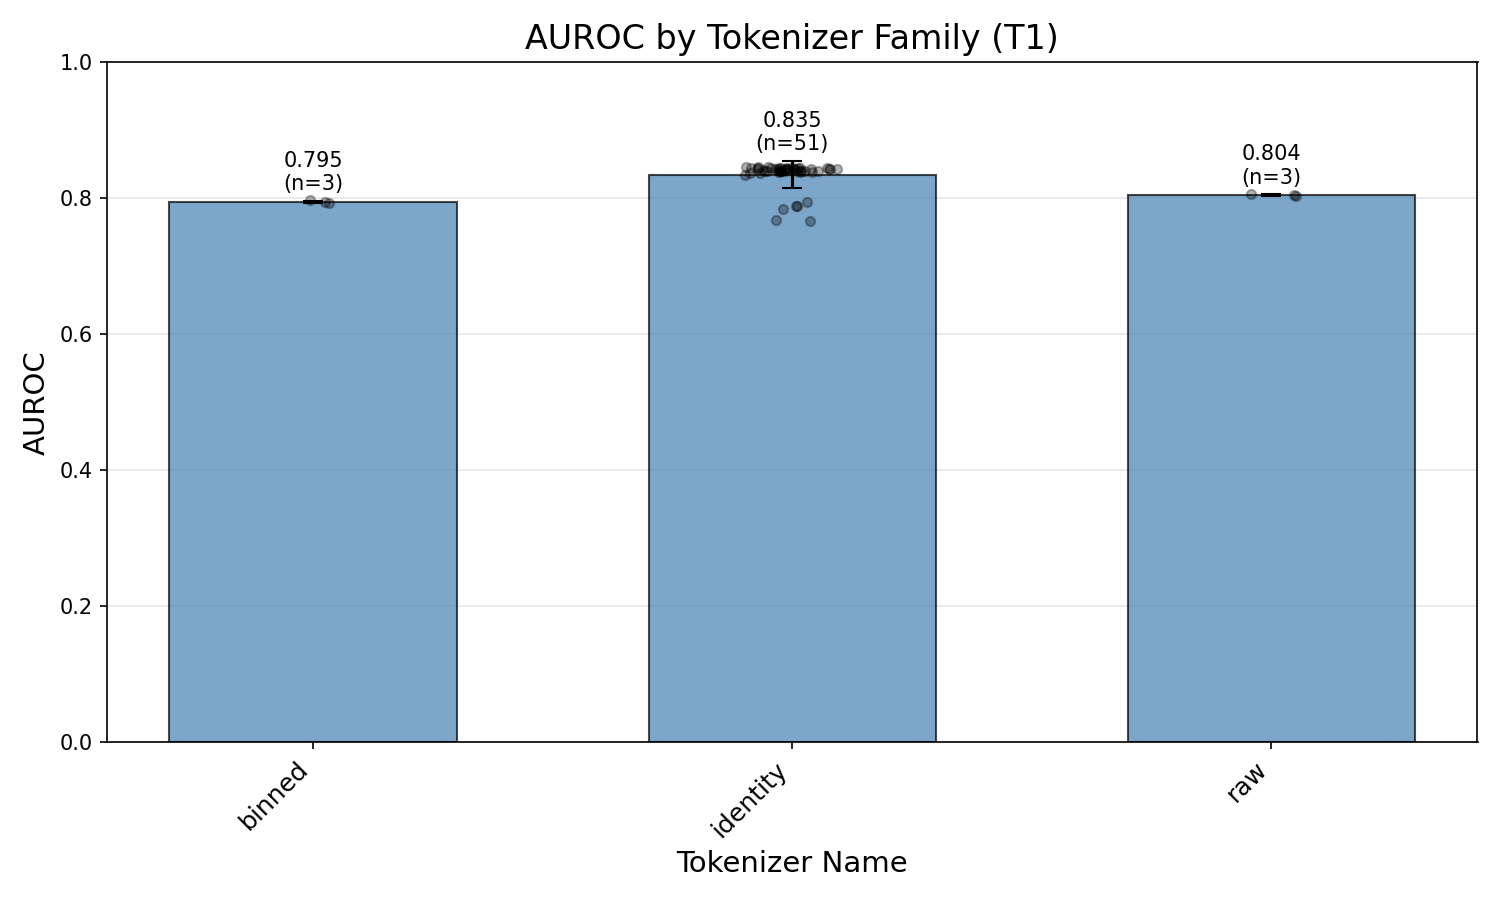
\includegraphics[width=0.65\textwidth]{figures/ch4/figure-auroc_bar_by_tokenizer.png}
\caption{Mean test AUROC by tokenizer family (T1).
Error bars show one standard deviation over seeds.
The \texttt{identity} family pools all T1-a and T1-b configurations ($n=51$);
\texttt{raw} and \texttt{binned} each have $n=3$ (three seeds).
% NOTE: consider regenerating with median + IQR, or separating identity
%   sub-configurations to avoid conflating the learned/dim=8 outlier.
}
\label{fig:auroc-bar-tokenizer}
\end{figure}

% [HAVE] Figure: ROC curves by tokenizer family
\begin{figure}[h]
\centering
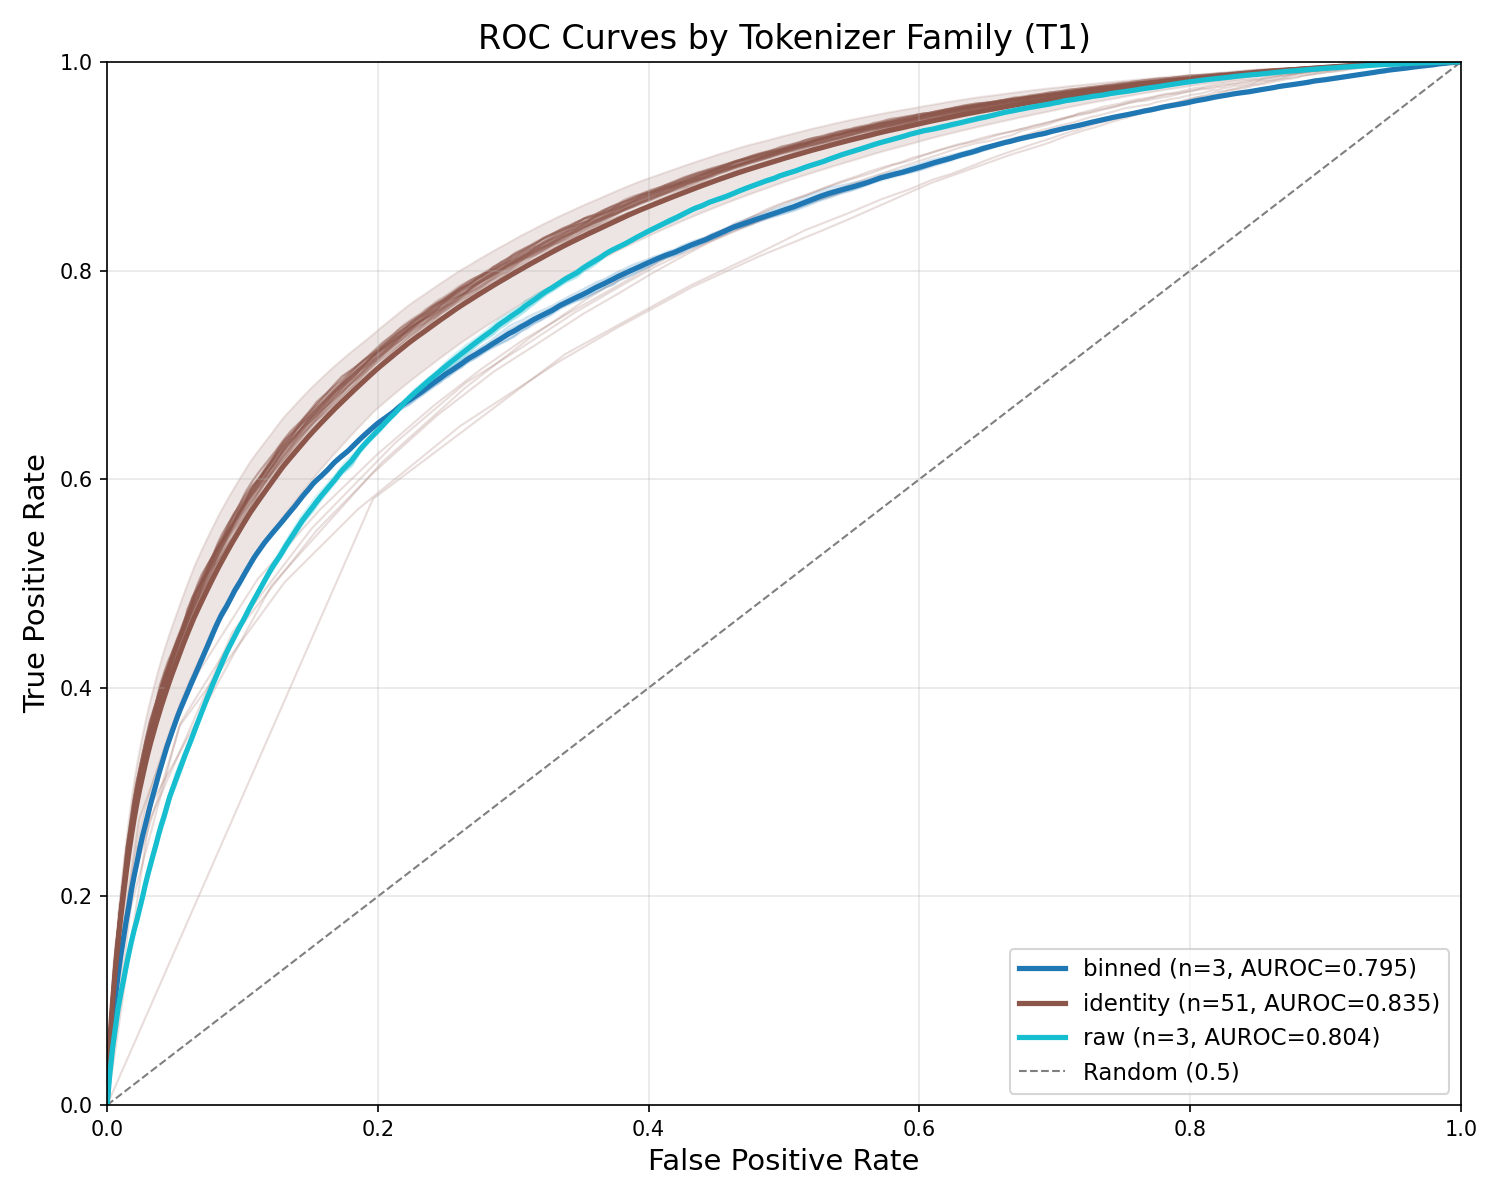
\includegraphics[width=0.65\textwidth]{figures/ch4/figure-roc_curves_by_tokenizer.png}
\caption{ROC curves by tokenizer family.
Shaded bands span the seed spread for \texttt{identity};
\texttt{raw} and \texttt{binned} show individual seed curves.
The identity advantage is uniform across the full operating range.}
\label{fig:roc-tokenizer}
\end{figure}

% [HAVE] Figure: validation AUROC training curves by tokenizer family
\begin{figure}[h]
\centering
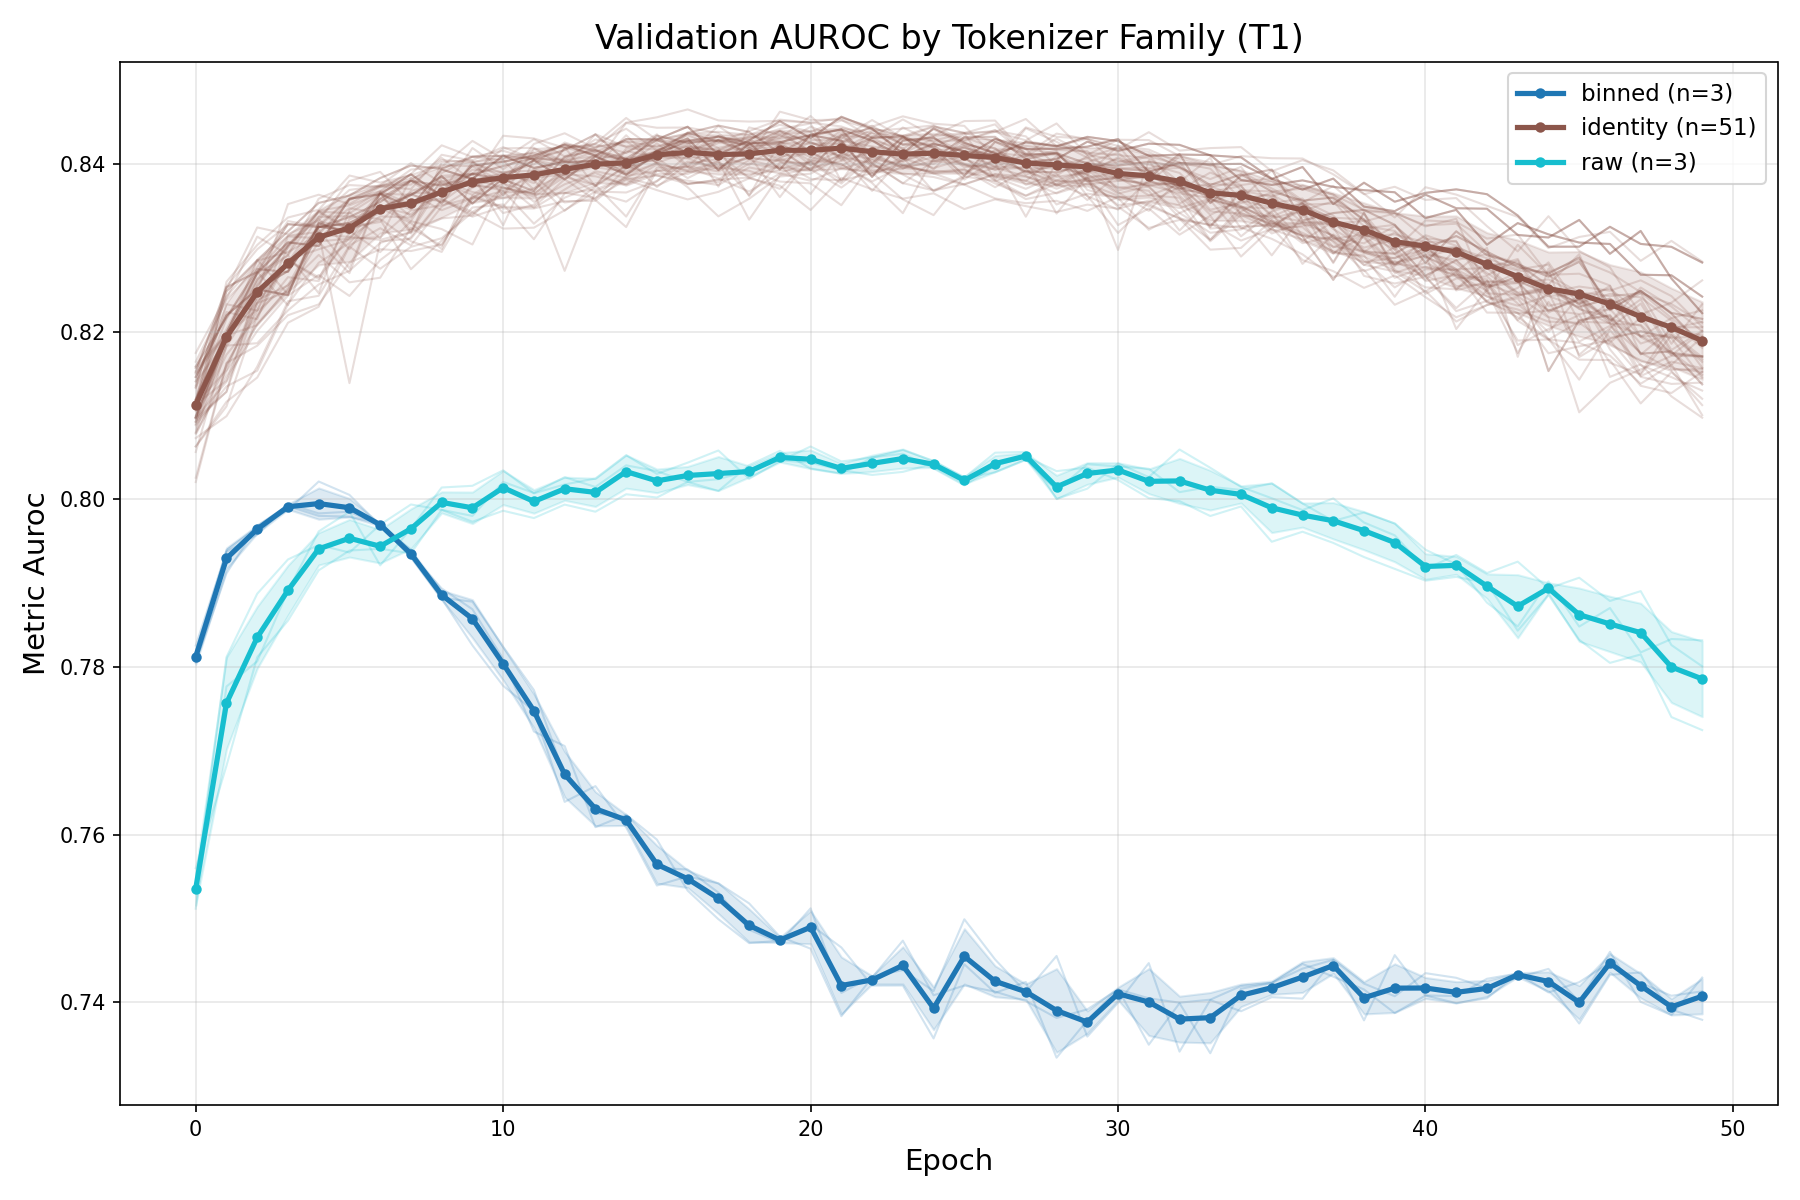
\includegraphics[width=0.65\textwidth]{figures/ch4/figure-val_auroc_by_tokenizer.png}
\caption{Validation AUROC over training epochs by tokenizer family.
\texttt{binned} peaks near epoch 4 and subsequently collapses, indicating
rapid overfitting once the discrete token vocabulary is memorised.
\texttt{raw} converges stably but at a lower plateau.
\texttt{identity} converges to a higher plateau and degrades slowly beyond
peak, consistent with mild overtraining at 50 epochs.
% NOTE: may want to crop x-axis to 0--35 epochs to focus on the interesting region.
}
\label{fig:val-auroc-tokenizer}
\end{figure}

% -------------------------------------------------------
\subsection{PID encoding mode and embedding dimension (T1-a, T1-b)}
\label{sec:exp4a-pid}
% -------------------------------------------------------

% --- NOTE ---
% This subsection has a trap in the data that must be explained honestly.
%
% The 1D bar for T1-a (Fig~\ref{fig:auroc-bar-pid-mode}) shows:
%   one_hot=0.844, fixed_random=0.841, learned=0.825.
% This naively reads as "learned is worse." But the heatmap
%   (Fig~\ref{fig:heatmap-pid-dim}) reveals the confound:
%   learned at dim=8 collapses to 0.8275, while at dim=16/32 it
%   recovers to 0.840+. The learned bar is depressed because dim=8
%   runs dominate the learned sample (n=39 vs n=9 for others).
%
% The fair comparison (all modes at dim=16 or dim=32) shows all three
%   modes within ~0.003 of each other.
%
% Interpretation: one_hot and fixed_random do not need to learn the
%   embedding geometry, so dim=8 is sufficient. Learned embeddings
%   at dim=8 are under-specified: 8 dimensions to learn a meaningful
%   geometry over the particle type vocabulary is tight, and optimisation
%   for the downstream task may sacrifice embedding quality.
%
% Practical conclusion: one_hot at dim=8 (or any dim, since one_hot is
%   dimension-agnostic by construction) is the most robust and parameter-efficient
%   choice. Use this as Ch5+ baseline.
%
% Write ~2 paragraphs: (1) explain the 1D bar trap, (2) read the heatmap correctly.

% [HAVE] Figure: AUROC bar by PID mode (1D marginal — misleading, needs caveat)
\begin{figure}[h]
\centering
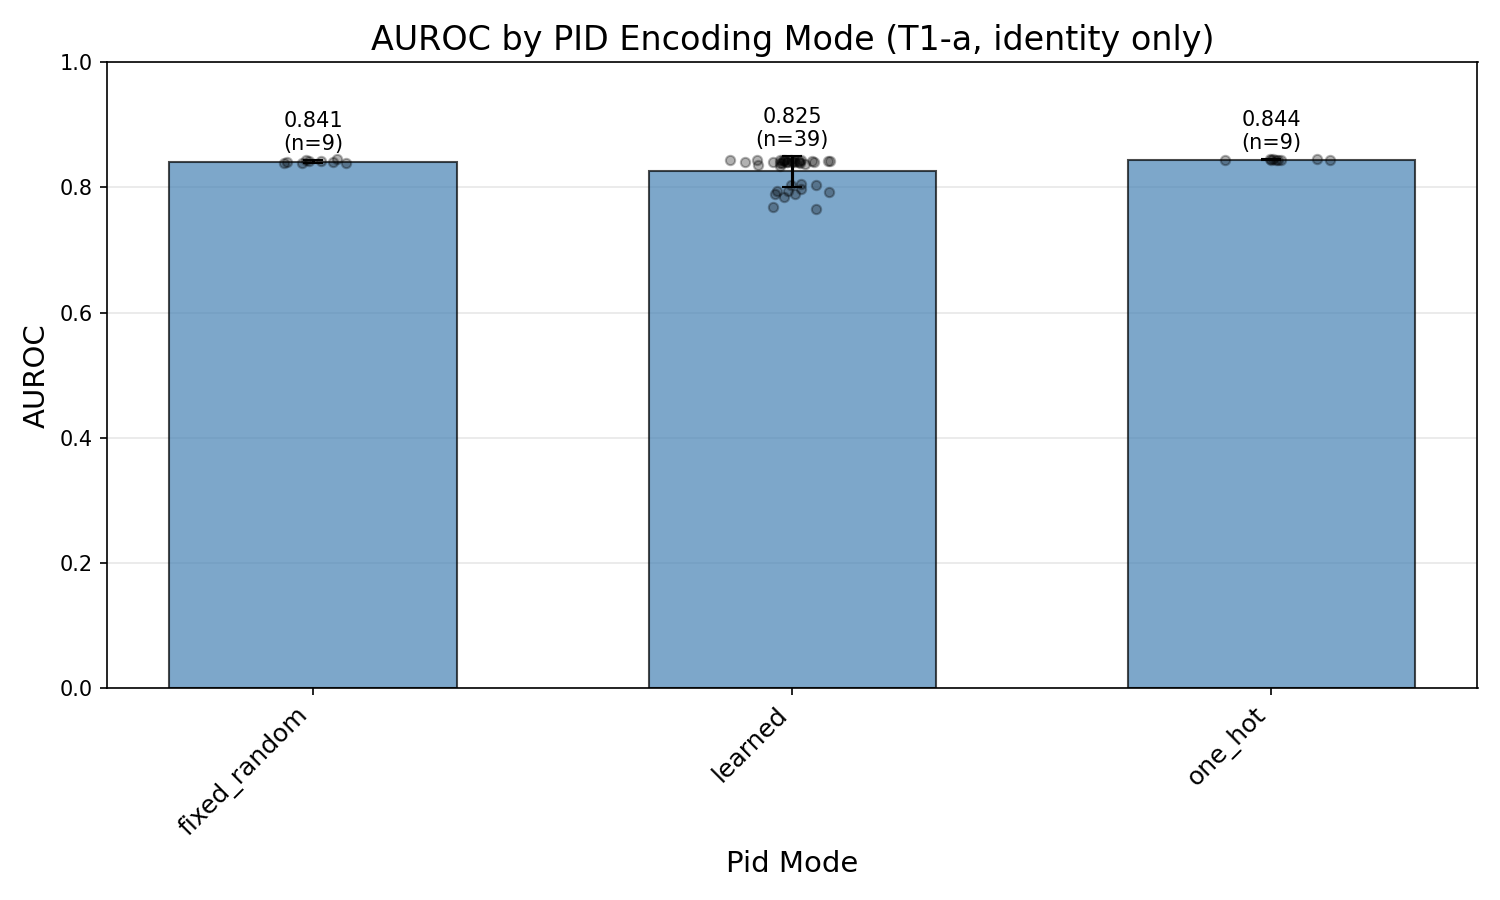
\includegraphics[width=0.65\textwidth]{figures/ch4/figure-auroc_bar_by_pid_mode.png}
\caption{Mean test AUROC by PID encoding mode (T1-a), pooled over all T1-b
embedding dimensions.
The apparent underperformance of \texttt{learned} is a confound:
the \texttt{learned} sample is dominated by dim=8 runs ($n=39$ of $n=57$),
which perform poorly (see Figure~\ref{fig:heatmap-pid-dim}).
At dim\,$\geq$\,16, all three modes are within $0.003$ AUROC of each other.
% NOTE: consider replacing this figure with one that holds dim fixed,
%   or annotating it with a dashed line for "learned at dim=16+."
}
\label{fig:auroc-bar-pid-mode}
\end{figure}

% [HAVE] Figure: AUROC heatmap T1-a x T1-b
\begin{figure}[h]
\centering
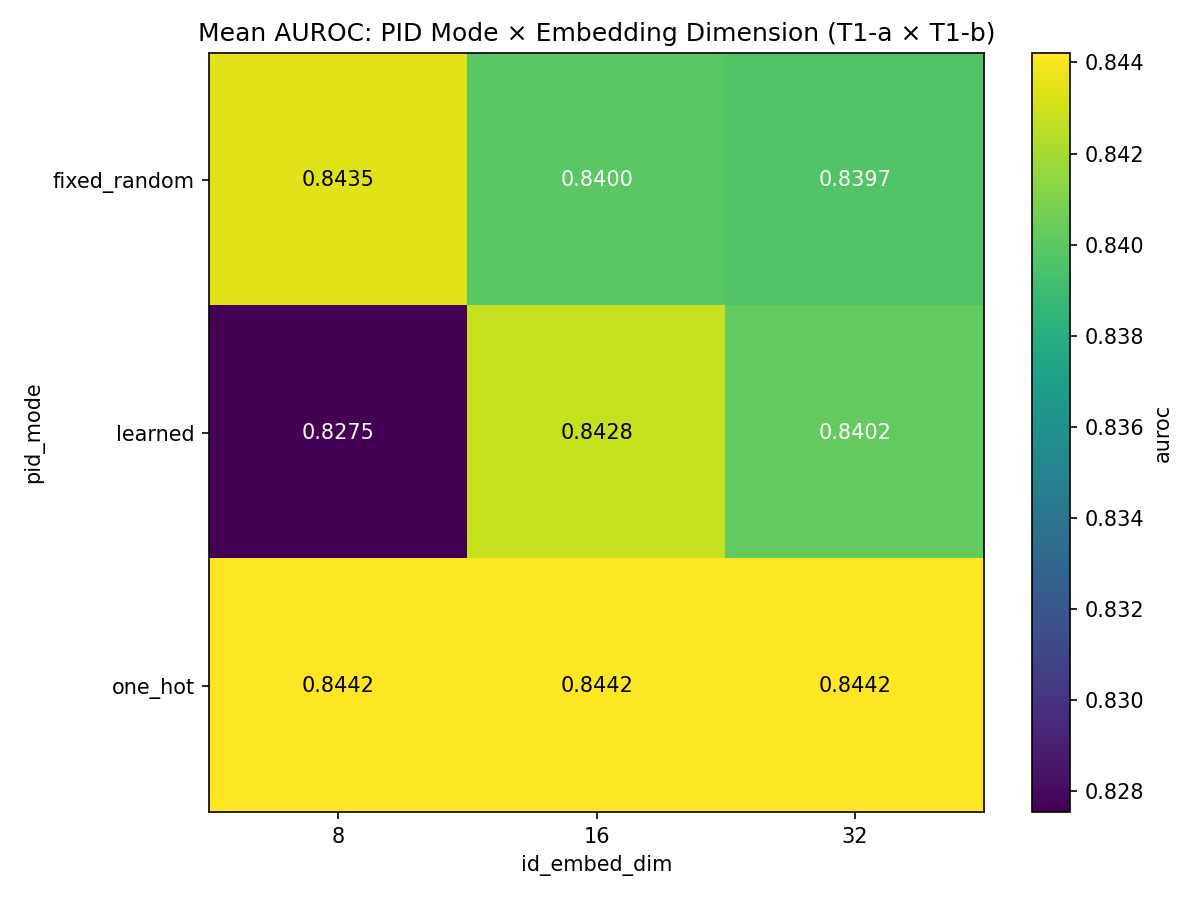
\includegraphics[width=0.72\textwidth]{figures/ch4/figure-auroc_heatmap_pid_mode_x_embed_dim.png}
\caption{Mean test AUROC as a function of PID encoding mode (T1-a) and
embedding dimension (T1-b), for the \texttt{identity} tokenizer family.
\texttt{one\_hot} is invariant to dimension by construction
(the embedding dimension is overridden to the number of particle types).
\texttt{fixed\_random} performs well at all dimensions.
\texttt{learned} at dim=8 is the clear outlier (0.8275);
at dim$\,\geq\,$16 it recovers to parity with the other modes.}
\label{fig:heatmap-pid-dim}
\end{figure}

% [HAVE] Figure: AUROC bar by embedding dimension (1D marginal)
\begin{figure}[h]
\centering
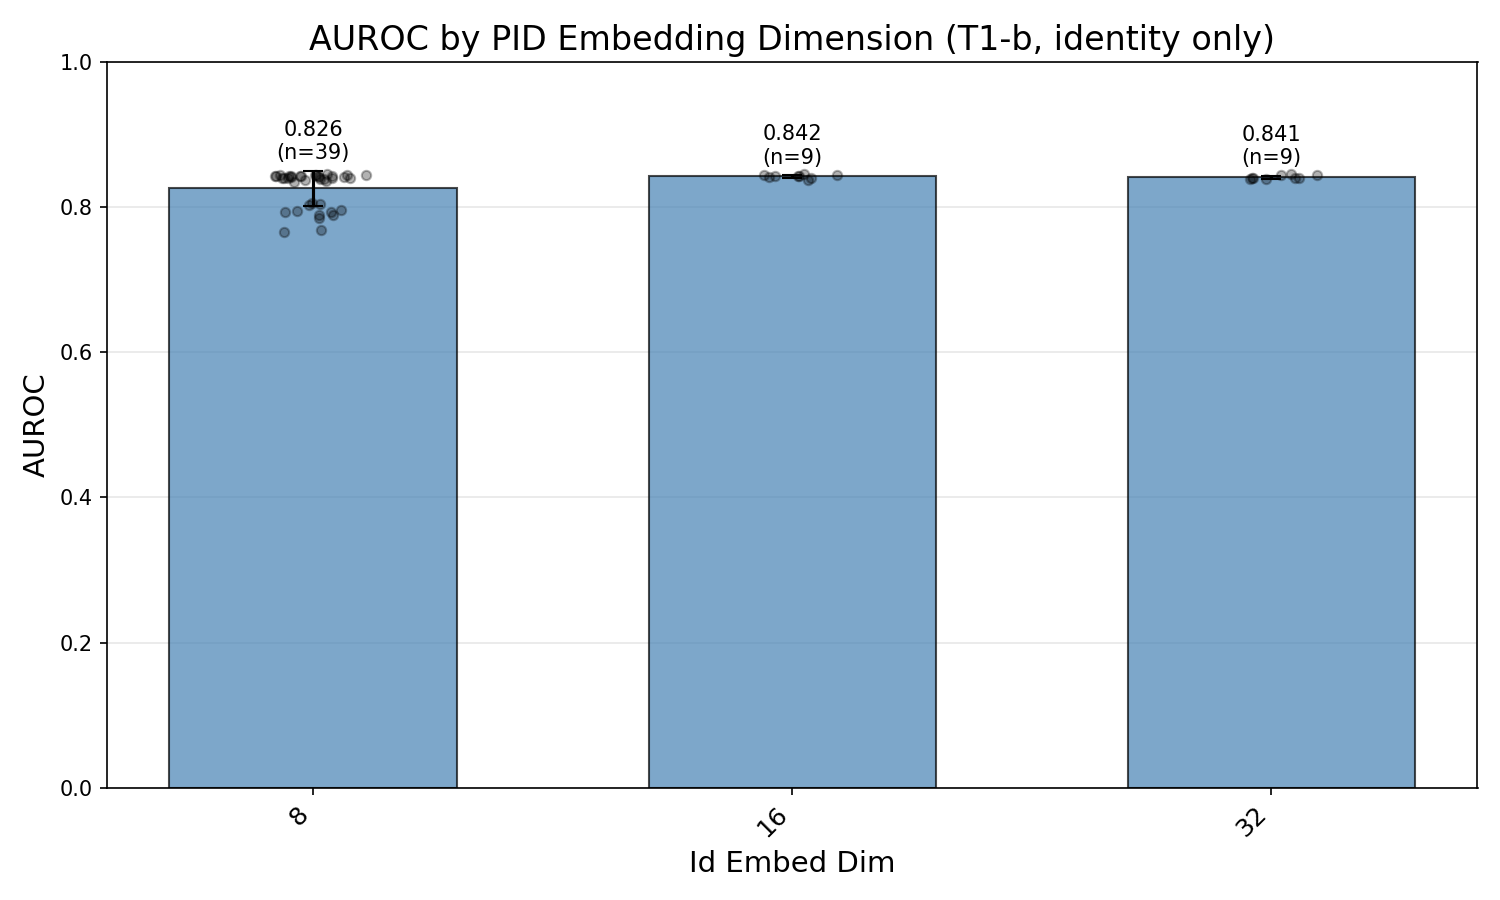
\includegraphics[width=0.65\textwidth]{figures/ch4/figure-auroc_bar_by_id_embed_dim.png}
\caption{Mean test AUROC by PID embedding dimension (T1-b), pooled over T1-a modes.
The dim=8 average ($0.826$) is depressed by the \texttt{learned}/dim=8 outlier.
Dim=16 ($0.842$) and dim=32 ($0.841$) are effectively equivalent.
% NOTE: same caveat as Fig~\ref{fig:auroc-bar-pid-mode}; this 1D view is
%   misleading without the heatmap context.
}
\label{fig:auroc-bar-dim}
\end{figure}

% [NEED] Optional figure: t-SNE or UMAP of the learned PID embedding vectors
%   coloured by particle type. Would show whether 8 dimensions produce
%   a collapsed/entangled geometry vs 16+ producing clean separation.
%   Low priority — only add if the geometry story is interesting.
% \begin{figure}[h]
% \centering
% \includegraphics[width=0.65\textwidth]{figures/ch4/figure-tsne_pid_embeddings.png}
% \caption{[PLACEHOLDER] t-SNE projection of learned PID embedding vectors
%   at dim=8 (left) and dim=16 (right), coloured by particle type.}
% \label{fig:tsne-pid}
% \end{figure}

% -------------------------------------------------------
\subsection{Failure analysis: what does PID unlock?}
\label{sec:exp4a-failure}
% -------------------------------------------------------

% --- NOTE ---
% This is the interpretability payoff of the chapter. Keep it tight.
%
% The failure analysis compares per-event predictions between the best
%   raw model and the best identity model on the held-out test set
%   (N=30,207 events).
%
% Numbers from the figure:
%   both_correct:   20,121  (66.6%)
%   identity_fixed: 2,515   (8.3%)  — PID helped
%   raw_fixed:      2,014   (6.7%)  — PID hurt
%   both_wrong:     5,557   (18.4%)
%   net gain:       +501 events
%
% Argument to make:
%   (1) The vast majority of events are correctly handled by both or neither.
%       PID changes the outcome for ~15% of events total.
%   (2) The net asymmetry (8.3% vs 6.7%) is real but modest. PID is not
%       universally helpful: in 6.7% of events, removing the explicit label
%       actually improves classification. This is worth one sentence of
%       explanation: those events may have ambiguous or mislabelled type
%       information, or the raw model learns a compensating heuristic.
%   (3) The scatter plot (left panel) shows that identity-fixed events
%       (blue) sit systematically above the diagonal — the identity model
%       pushes them toward higher signal score. The raw-fixed events (orange)
%       sit below.
%   (4) 18.4% of events are wrong for both: these define the irreducible
%       difficulty ceiling of the task regardless of tokenizer.
%
% [WANT] An additional breakdown: of the 2,515 events where PID helped,
%   what is their kinematic profile? Hypothesis: they are events where
%   particle type is ambiguous from kinematics (e.g., b-jets and light jets
%   at similar pT). If the report already extracted event-level features for
%   the flipped events, this could be a simple 1D histogram of, e.g.,
%   jet multiplicity or leading jet pT for the four categories.
%   Flag for potential new inference run if not available.

Of the $30{,}207$ test events,
$66.6\%$ are classified correctly by both tokenizers,
and $18.4\%$ are wrong for both,
defining the task's irreducible floor given this model capacity and data.
In the remaining $15\%$,
the tokenizer choice determines the outcome:
$8.3\%$ of events are fixed by adding an explicit particle-type label
(PID helped),
while $6.7\%$ are misclassified when PID is available but correct without it
(PID hurt),
giving a net gain of $501$ events.

\begin{figure}[h]
\centering
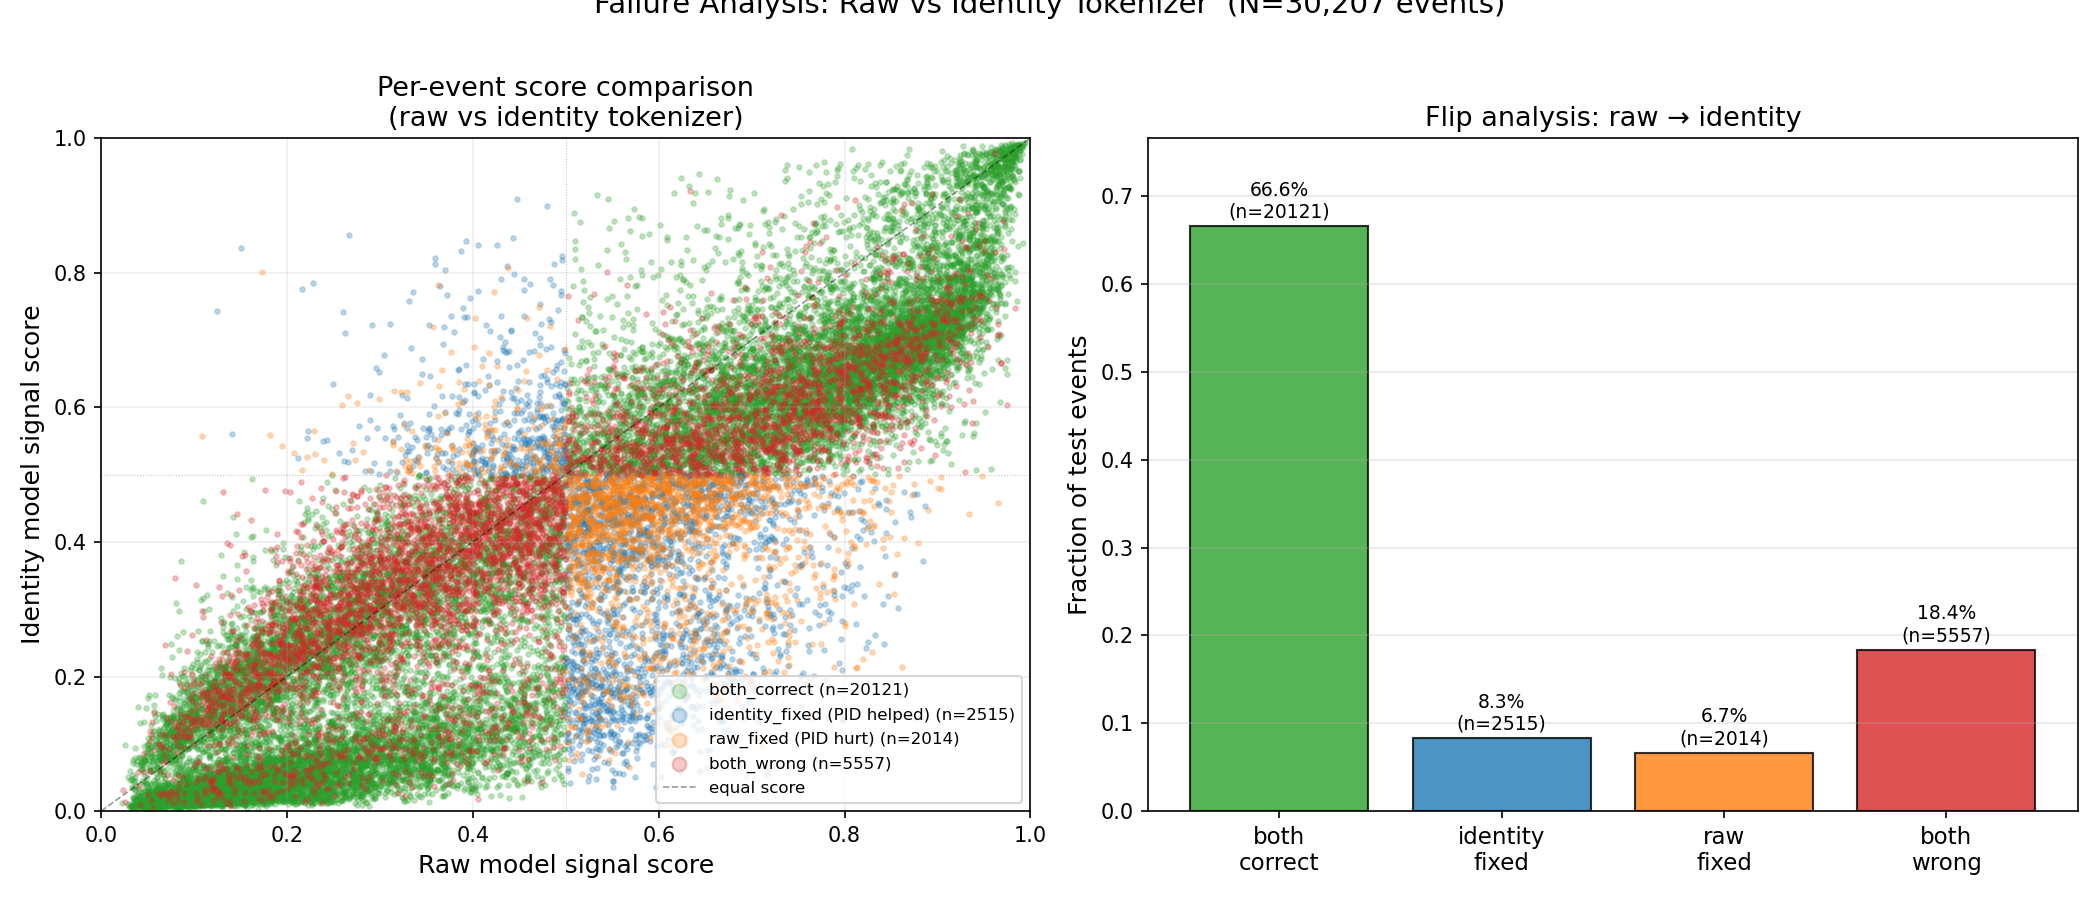
\includegraphics[width=\textwidth]{figures/ch4/figure-failure_analysis_raw_vs_identity.png}
\caption{Failure analysis comparing per-event classifier scores for the
\texttt{raw} (x-axis) and \texttt{identity} (y-axis) tokenizers on the
test set ($N=30{,}207$ events).
\textit{Left:} scatter of per-event signal scores; colours indicate outcome category.
\textit{Right:} fraction of events in each category.
Events above the diagonal benefit from the explicit PID label;
events below are hurt by it.
% NOTE: a follow-up plot breaking down the "identity_fixed" and "raw_fixed"
%   populations by kinematic variables (e.g. jet multiplicity, b-jet pT)
%   would strengthen the interpretability argument. Flag for additional inference.
}
\label{fig:failure-analysis}
\end{figure}

% ============================================================
\section{Feature content and token ordering (Exp.\ 4B)}
\label{sec:exp4b}
% ============================================================

% --- SECTION INTRO NOTE ---
% 1 short paragraph: fix T1=identity, T1-a=one_hot (or learned+dim=16),
%   T1-b=8 (for one_hot). Then ask three independent questions about
%   what information the tokens carry: D01 (energy), D02 (MET), D03 (order).
%   Refer to Table~\ref{tab:exp4b}.

\begin{table}[h]
\centering
\small
\begin{tabular}{lllr}
\toprule
Factor & Axis & Values & $n_\text{configs}$ \\
\midrule
Feature set & D01 & \texttt{[0,1,2,3]} $\cdot$ \texttt{[1,2,3]} & 2 \\
MET included & D02 & \texttt{false} $\cdot$ \texttt{true} & 2 \\
Token order & D03 & \texttt{input\_order} $\cdot$ \texttt{shuffled} & 2 \\
\midrule
\multicolumn{3}{l}{Unique configurations ($2^3$)} & 8 \\
\multicolumn{3}{l}{Seeds per configuration} & 3 \\
\multicolumn{3}{l}{\textbf{Total runs}} & \textbf{24} \\
\bottomrule
\end{tabular}
\caption{Experiment 4B sweep design.
Fixed: T1\,=\,\texttt{identity}, T1-a\,=\,\texttt{one\_hot}, T1-b\,=\,8.
% NOTE: confirm whether Exp 4B was actually run with one_hot or learned.
%   If learned+dim=8, the baseline AUROC will be depressed relative to the
%   best identity configuration. Cross-check against run configs before finalising.
}
\label{tab:exp4b}
\end{table}

% -------------------------------------------------------
\subsection{Energy inclusion (D01)}
\label{sec:exp4b-energy}
% -------------------------------------------------------

% --- NOTE ---
% Numbers: all_features (E,pT,η,φ) = 0.835 vs no_energy (pT,η,φ) = 0.826.
%   Gap = -0.009 AUROC when energy is dropped.
%
% Argument:
%   (1) Physics lens: energy E is not Lorentz-invariant, but it encodes mass
%       information via m² = E² - |p|². For top quark decay products
%       (W bosons, b-jets), the invariant masses of sub-systems are powerful
%       discriminants. Dropping E removes the model's ability to reconstruct
%       these masses implicitly.
%   (2) ML lens: the gap is modest (0.009), suggesting the model partially
%       compensates using the remaining three features. At fixed η, the
%       relationship E ≈ pT·cosh(η) holds for massless particles, so pT and η
%       together recover most of E for light jets and photons. The residual
%       gap reflects the genuinely mass-sensitive component.
%   (3) Practical conclusion: include energy (D01 = [0,1,2,3]) in the baseline.
%
% 2 sentences of argument + figure.

Removing the energy component (D01\,=\,\texttt{[1,2,3]}) reduces mean AUROC
by $0.009$ relative to the full four-vector (D01\,=\,\texttt{[0,1,2,3]},
AUROC\,=\,$0.835$).

\begin{figure}[h]
\centering
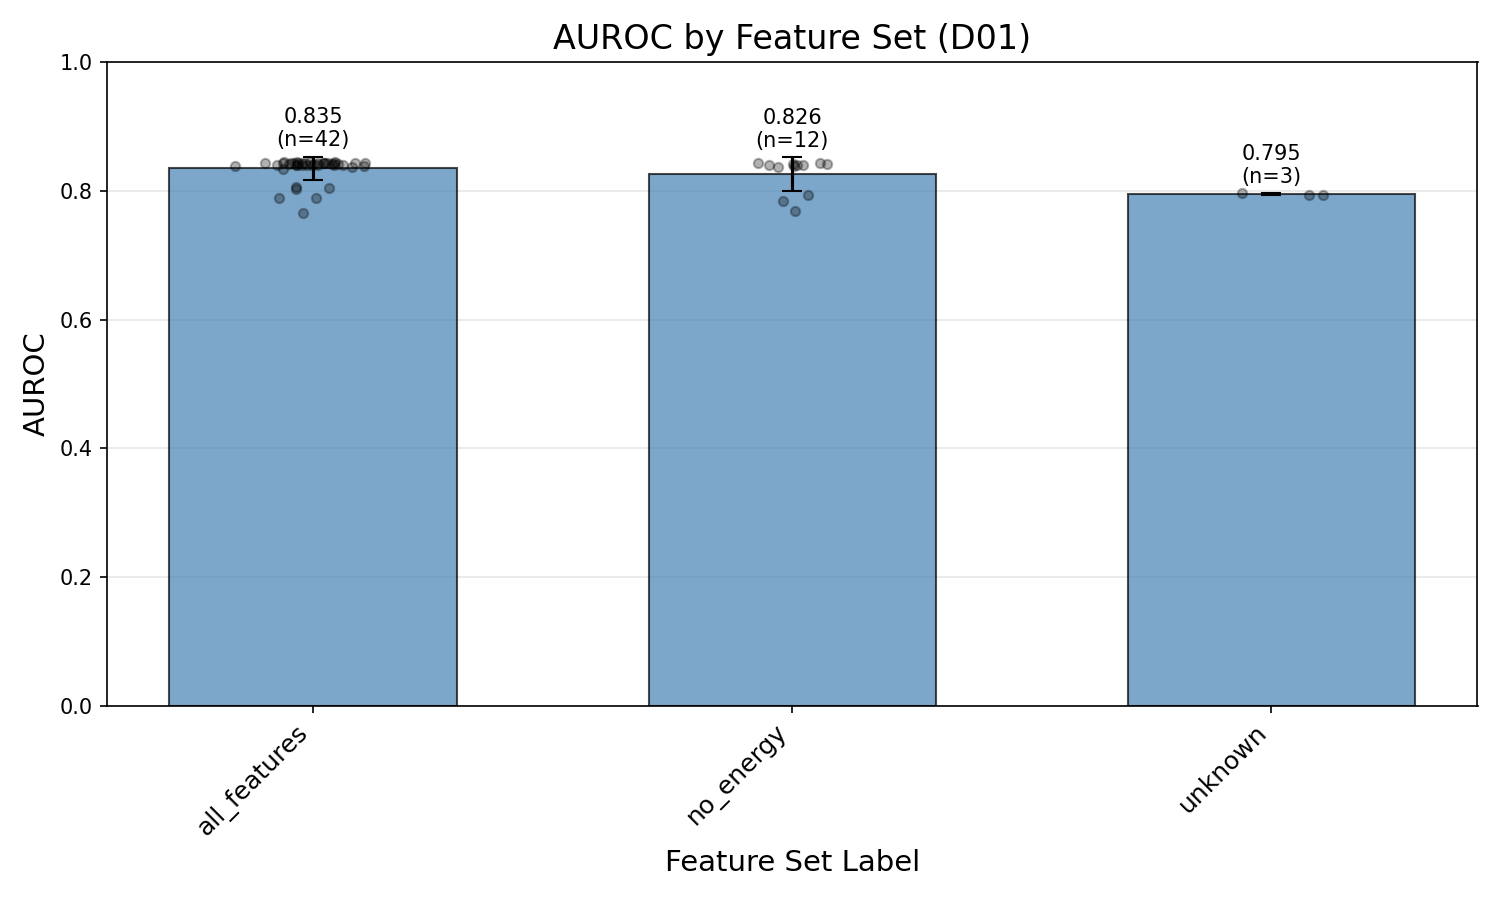
\includegraphics[width=0.65\textwidth]{figures/ch4/figure-auroc_bar_by_features.png}
\caption{Mean test AUROC by feature set (D01).
\texttt{all\_features}: $(E, p_T, \eta, \phi)$;
\texttt{no\_energy}: $(p_T, \eta, \phi)$.
The \texttt{unknown} bar corresponds to the \texttt{binned} tokenizer runs,
where continuous features are not directly accessible, included for completeness.
% NOTE: the "unknown" bar is confusing. Consider either dropping it or
%   relabelling it explicitly as "binned (no continuous features)".
%   Also consider adding a horizontal reference line at raw AUROC = 0.804
%   to contextualise the energy gap.
}
\label{fig:auroc-bar-features}
\end{figure}

% -------------------------------------------------------
\subsection{Missing transverse energy (D02)}
\label{sec:exp4b-met}
% -------------------------------------------------------

% --- NOTE ---
% Numbers: without MET = 0.836, with MET = 0.810. Gap = -0.026.
%   This is a NEGATIVE result: MET HURTS.
%
% This needs honest treatment. Three candidate explanations:
%
%   (A) PE-confusion hypothesis (leading candidate):
%       The sinusoidal positional encoding (E1=sinusoidal, positional_space=model)
%       is active in these runs. Token position carries a signal (as shown
%       by D03 below). MET is appended as an additional token at a fixed
%       position. If attention patterns have learned to associate position
%       with particle type, inserting a MET token at a fixed slot disrupts
%       those patterns for all other tokens.
%
%   (B) Noise injection:
%       MET reconstruction in high-multiplicity events (≥8 jets + leptons)
%       has large experimental resolution. The MET token may carry more
%       noise than signal, particularly for the 4t-vs-bg task where the
%       MET significance varies strongly across background processes.
%
%   (C) Interaction with D03:
%       If the D02=true runs were all run with input_order (D03=false),
%       the MET token appears at a fixed position, compounding hypothesis A.
%       Cross-check: does MET still hurt when D03=shuffled? If the gap
%       disappears under shuffling, hypothesis A is confirmed.
%       [FLAG: this cross-check may require a targeted additional run of
%        ~6 configurations: D02=true × D03=shuffled × 3 seeds.]
%
% Practical conclusion for Ch5+: D02=false. MET is revisited in Ch5
%   where physics-informed attention biases (B1-G1=met_direction) provide
%   a more principled way to inject MET information.
%
% Write ~2 paragraphs: (1) state the result; (2) discuss the explanation
%   candidates. Keep the D03 cross-check as a parenthetical or footnote.

Contrary to the expectation that missing transverse energy provides
additional signal from the neutrino system,
including MET as a token (D02\,=\,\texttt{true}) reduces mean AUROC
by $0.026$ relative to the MET-free baseline ($0.836$ vs $0.810$).

\begin{figure}[h]
\centering
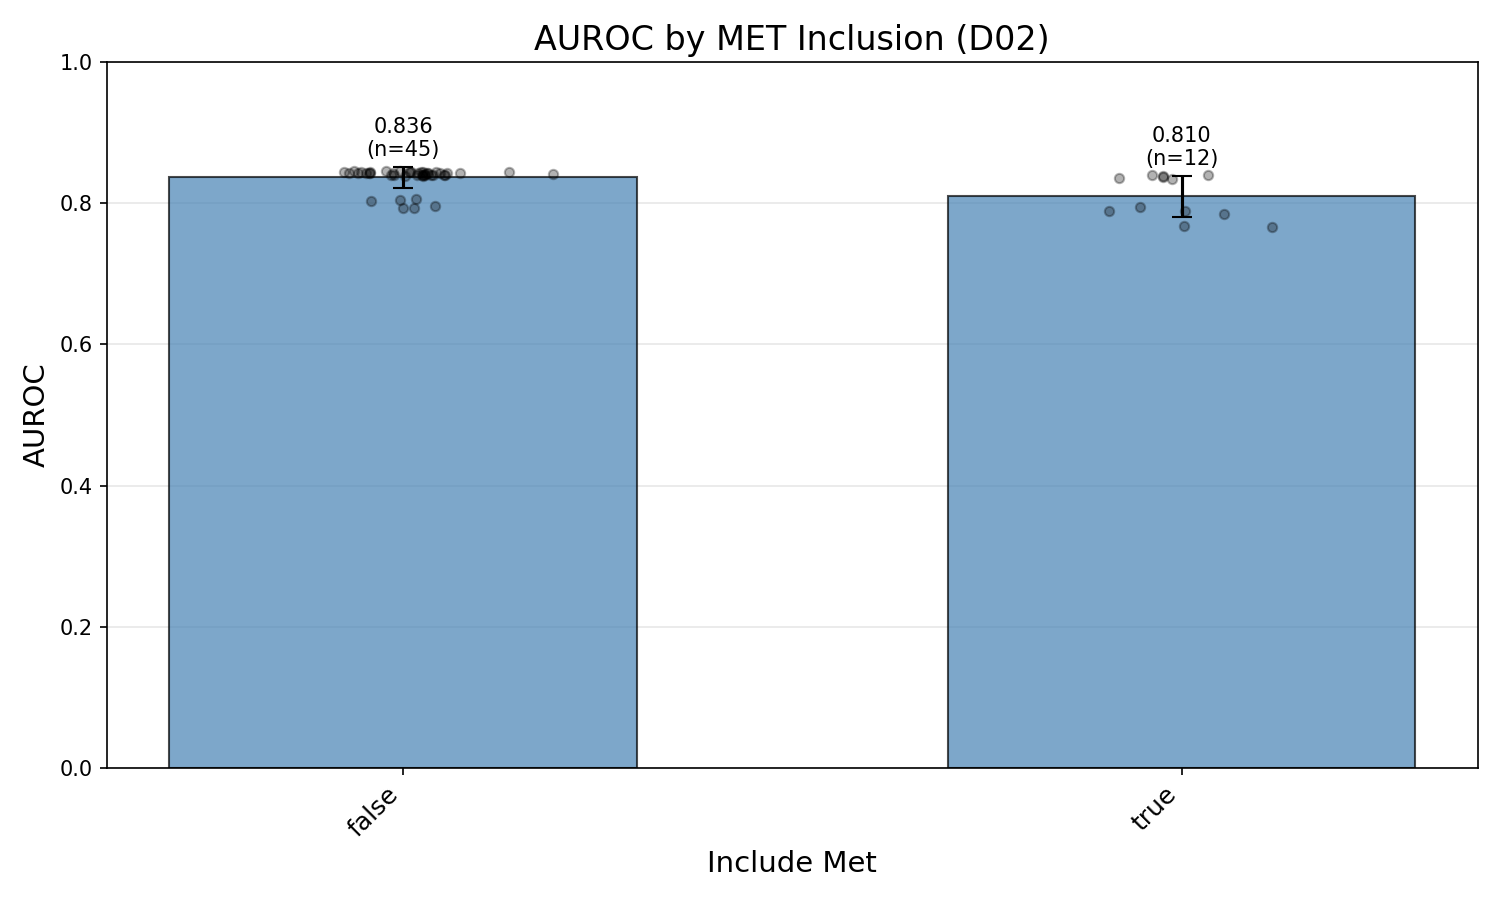
\includegraphics[width=0.65\textwidth]{figures/ch4/figure-auroc_bar_by_met.png}
\caption{Mean test AUROC by MET inclusion (D02).
Including MET as a token degrades performance by $0.026$ AUROC on the
4t-vs-background task.
% NOTE: if the D03 cross-check runs are available (D02=true × D03=shuffled),
%   add a second grouped bar showing MET effect separately for ordered and
%   shuffled conditions. This is the key diagnostic for the PE-confusion hypothesis.
}
\label{fig:auroc-bar-met}
\end{figure}

% [NEED] Figure: MET effect stratified by D03 ordering condition
%   (to test PE-confusion hypothesis). Requires ~6 additional runs.
% \begin{figure}[h]
% \centering
% \includegraphics[width=0.65\textwidth]{figures/ch4/figure-auroc_met_by_ordering.png}
% \caption{[PLACEHOLDER] Mean test AUROC as a function of MET inclusion (D02),
%   shown separately for ordered (D03=input\_order) and shuffled (D03=shuffled)
%   token sequences. If the MET penalty disappears under shuffling, the
%   PE-confusion hypothesis is confirmed.}
% \label{fig:auroc-met-by-ordering}
% \end{figure}

% -------------------------------------------------------
\subsection{Token ordering as a permutation-invariance diagnostic (D03)}
\label{sec:exp4b-order}
% -------------------------------------------------------

% --- NOTE ---
% Numbers: input_order = 0.840, shuffled = 0.811. Gap = -0.029.
%
% This is the second surprise. Self-attention is permutation-equivariant
%   by construction (no positional encoding → truly order-invariant).
%   But all these runs use E1=sinusoidal with positional_space=model.
%   Sinusoidal PE injects an ordering signal. If the input ordering has
%   any physical structure (e.g., particles ordered by reconstruction
%   algorithm output, or by pT descending), the PE effectively becomes
%   a pT-proxy or type-proxy.
%
% Consequence: the -0.029 gap does NOT mean the attention mechanism is
%   exploiting ordering. It means the sinusoidal PE is exploiting ordering.
%   True permutation invariance requires E1=none.
%
% This result does two things for the thesis:
%   (1) It closes the chapter with a concrete negative finding that
%       motivates the positional encoding chapter (if one exists) or
%       at minimum serves as a caveat for all PE=sinusoidal results.
%   (2) It means that for any future chapter, D03=input_order is the
%       correct default (not shuffled), since the model uses the ordering.
%       But the physics meaning of that ordering should be checked.
%
% [FLAG: check what ordering the reconstruction software produces.
%   If it is pT-descending, the PE is effectively encoding pT rank,
%   which is a legitimate (if implicit) physics feature. If it is
%   arbitrary, the PE may be encoding noise.]
%
% Write ~2 paragraphs: (1) state the result and why it is surprising;
%   (2) explain the PE mechanism and what it implies for subsequent chapters.

Shuffling the token sequence (D03\,=\,\texttt{shuffled}) reduces mean AUROC
from $0.840$ to $0.811$ ($-0.029$),
despite self-attention being permutation-equivariant by construction.

\begin{figure}[h]
\centering
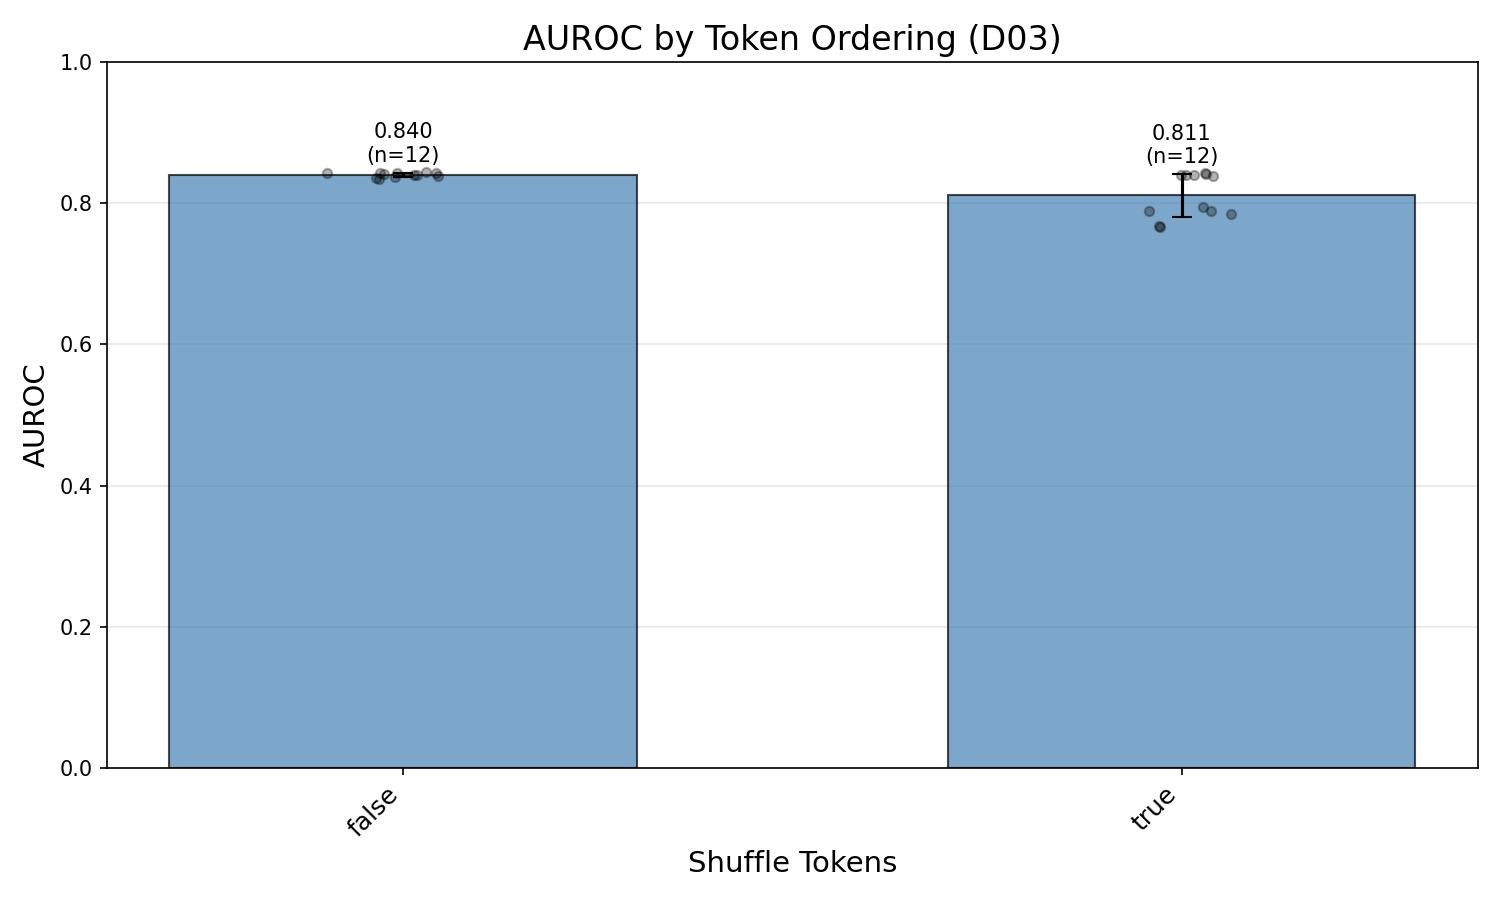
\includegraphics[width=0.65\textwidth]{figures/ch4/figure-auroc_bar_by_shuffle.png}
\caption{Mean test AUROC by token ordering (D03).
The performance gap under shuffling ($-0.029$) indicates that the sinusoidal
positional encoding (E1\,=\,\texttt{sinusoidal}) is exploiting the input
ordering of the particle sequence.
True permutation invariance would require E1\,=\,\texttt{none}.
% NOTE: if the report generates a val_auroc_by_shuffle training curve,
%   include it here to show whether shuffled models converge differently
%   or simply plateau lower.
}
\label{fig:auroc-bar-shuffle}
\end{figure}

% [NEED] Figure: training curves D03=ordered vs shuffled
%   (does shuffled model converge differently or just plateau lower?)
% \begin{figure}[h]
% \centering
% 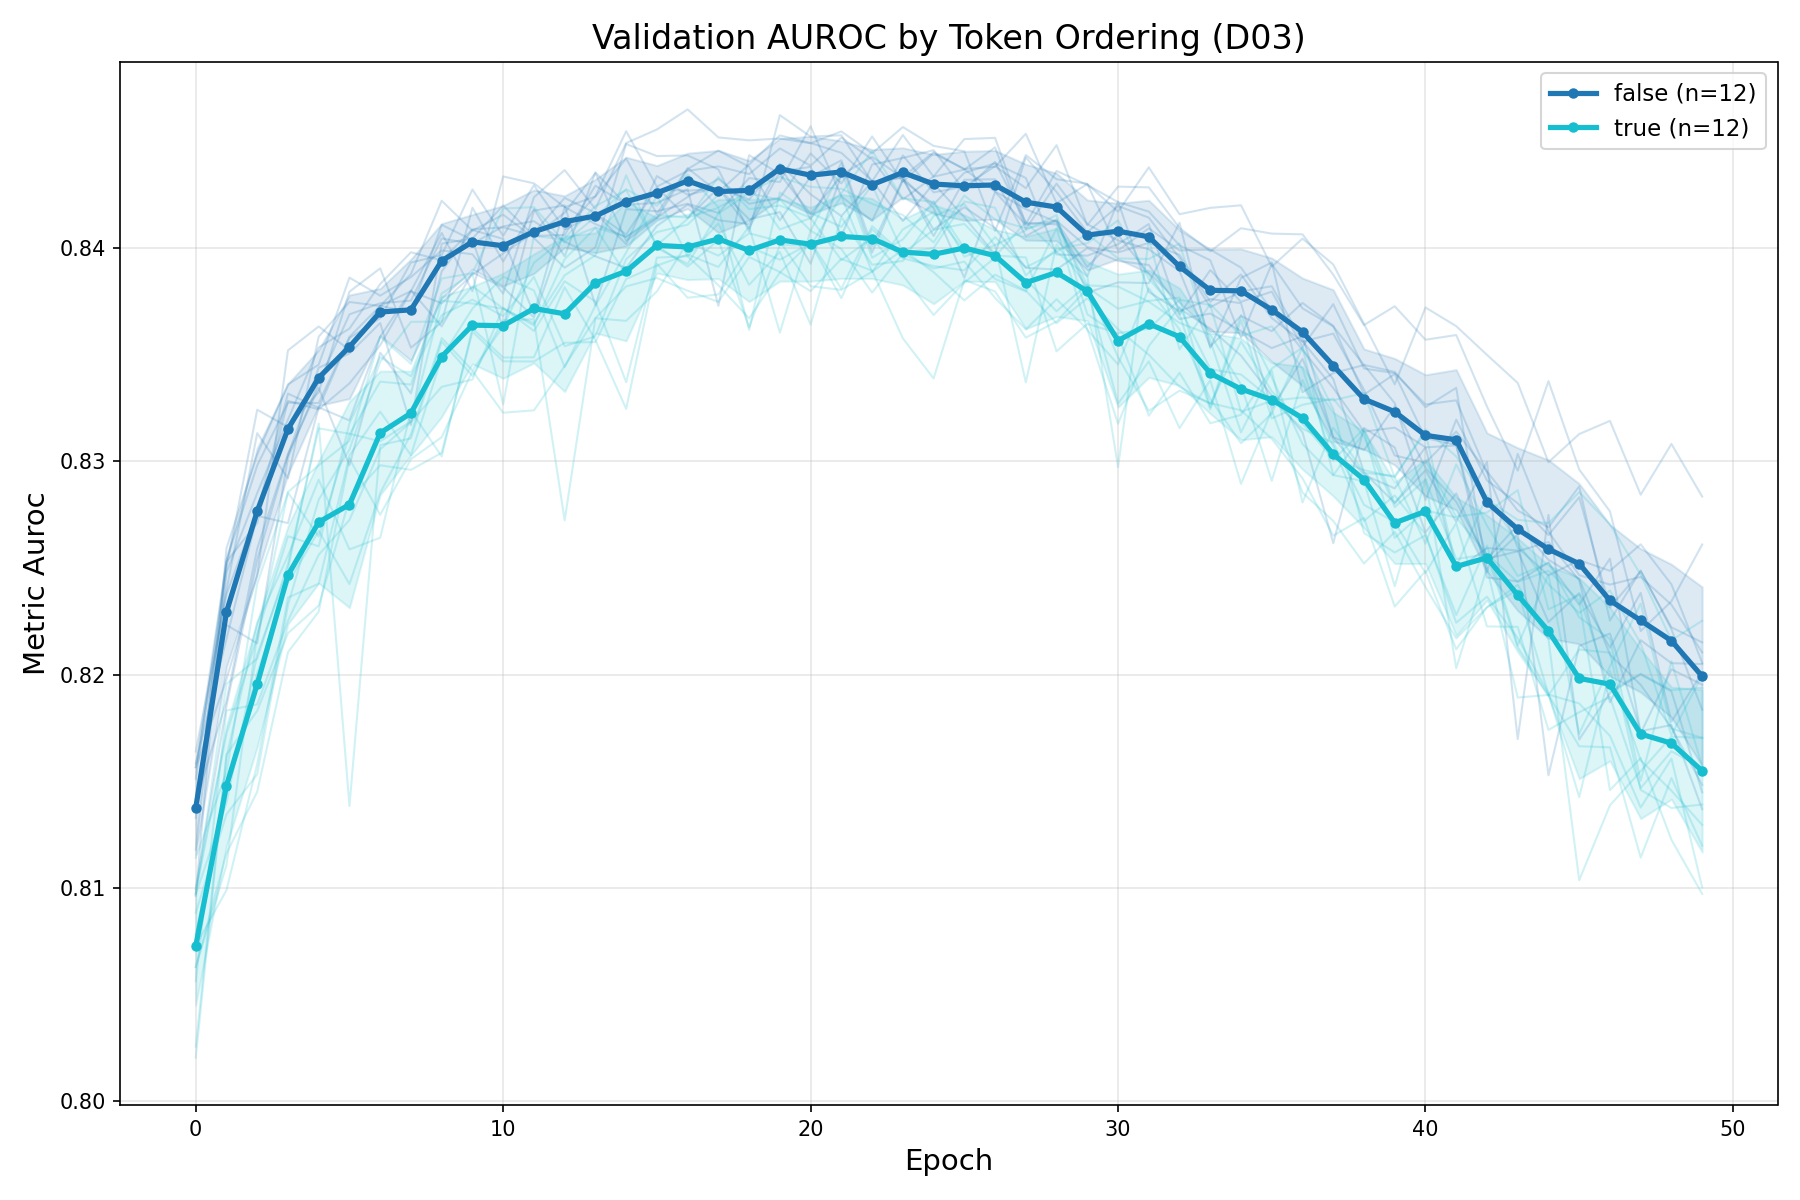
\includegraphics[width=0.65\textwidth]{figures/ch4/figure-val_auroc_by_shuffle.png}
% \caption{[PLACEHOLDER] Validation AUROC training curves for ordered vs
%   shuffled token sequences.}
% \label{fig:val-auroc-shuffle}
% \end{figure}

% [NEED] Figure: AUROC as function of D03, stratified by E1 (PE type),
%   specifically comparing E1=sinusoidal vs E1=none.
%   This would confirm that the shuffle penalty disappears when PE=none.
%   Requires ~6 additional runs: E1=none × D03=shuffled/ordered × 3 seeds.
%   Medium priority — useful for the PE chapter but also here.
% \begin{figure}[h]
% \centering
% \includegraphics[width=0.65\textwidth]{figures/ch4/figure-auroc_shuffle_by_pe.png}
% \caption{[PLACEHOLDER] Shuffle penalty as a function of positional encoding type.
%   E1=none should show no ordering effect; E1=sinusoidal should reproduce
%   the $-0.029$ gap observed here.}
% \label{fig:auroc-shuffle-by-pe}
% \end{figure}

% ============================================================
\section{Summary and chapter baseline}
\label{sec:ch4-summary}
% ============================================================

% --- NOTE ---
% Short section (~1 paragraph + table). State the three main findings:
%   (1) PID is load-bearing: the transformer cannot recover particle
%       identity from kinematics alone at this capacity. +0.031 AUROC.
%   (2) How PID is encoded matters only at low embedding dimension:
%       at dim≥16, all encoding modes are equivalent. one_hot at dim=8
%       is the parameter-efficient choice.
%   (3) Two counterintuitive negatives: MET hurts (-0.026) and shuffling
%       hurts (-0.029). Both implicate the sinusoidal positional encoding,
%       which is exploiting input ordering and may be disrupted by an
%       additional fixed-position MET token.
%
% Then: Table~\ref{tab:ch4-baseline} stating the chosen values for each
%   axis, with a one-line justification for each.
%
% Final sentence: these choices constitute the Ch5 baseline. Any subsequent
%   chapter that changes one of these axes re-runs the relevant comparison
%   on top of this configuration.

This chapter establishes six axis choices that propagate as the fixed baseline
into all subsequent chapters.
Three main conclusions motivate these choices.

First, an explicit particle-type label is necessary:
the \texttt{identity} tokenizer outperforms kinematics-only \texttt{raw}
by $+0.031$ AUROC,
and the failure analysis shows that this gap is concentrated in events
where particle type, not kinematics, carries the discriminating signal.
The \texttt{binned} tokenizer, which discards continuous features entirely,
is the weakest of the three families.

Second, the choice of PID encoding mode (T1-a) is largely irrelevant
provided the embedding dimension is at least 16 for the \texttt{learned} mode.
The \texttt{one\_hot} encoding at dimension 8 is robust and parameter-efficient,
making it the preferred baseline.

Third, two results indicate that the sinusoidal positional encoding (E1)
is a confounding variable in this chapter.
MET inclusion degrades performance ($-0.026$), most likely because the MET token
disrupts the attention patterns that the model has learned to associate with
input token position.
Similarly, shuffling the token sequence degrades performance ($-0.029$),
demonstrating that the model exploits the input ordering via the positional encoding
rather than being genuinely permutation-invariant.
Both effects point to the positional encoding as an implicit inductive bias
whose interaction with physics-motivated design choices warrants further study.

\begin{table}[h]
\centering
\small
\begin{tabular}{llll}
\toprule
Axis & Config key & Chosen value & Justification \\
\midrule
T1   & \texttt{tokenizer.name}     & \texttt{identity}    & $+0.031$ over \texttt{raw} \\
T1-a & \texttt{tokenizer.pid\_mode} & \texttt{one\_hot}    & robust at dim=8; no learning needed \\
T1-b & \texttt{tokenizer.id\_embed\_dim} & 8           & sufficient for \texttt{one\_hot} \\
D01  & \texttt{data.cont\_features} & \texttt{[0,1,2,3]}  & $+0.009$ from energy inclusion \\
D02  & \texttt{include\_met}        & \texttt{false}       & MET token degrades AUROC \\
D03  & \texttt{shuffle\_tokens}     & \texttt{false}       & model exploits input ordering \\
\bottomrule
\end{tabular}
\caption{Chapter 4 baseline configuration carried forward to all subsequent chapters.
% NOTE: T1-a choice may need revisiting if the planned cross-task (4t-vs-ttH)
%   results show a different ranking. Confirm before freezing.
}
\label{tab:ch4-baseline}
\end{table}

% [NEED] Cross-task validation subsection (or box):
%   Re-run T1 and D02 comparisons on the 4t-vs-ttH task.
%   Expected: T1 finding replicates (identity still best).
%   D02: on 4t-vs-ttH both signal and background have semi-leptonic tops,
%   so MET provides even less discriminating power, and the negative
%   result should be as strong or stronger.
%   6--12 additional runs. Include as a subsection if results are available;
%   otherwise move to an appendix or footnote.
%
% \subsection{Cross-task validation on $tttt$ vs $ttH$ (optional)}
% \label{sec:ch4-crosstask}
% [PLACEHOLDER: 1 figure, ~1 paragraph]
